\section{The Target Metamodel}
\label{sec:targetmetamodel}

The target metamodel is the language the model-to-model transformation of Task 2
writes into, and the language the code generation of Task 3 reads. It holds
every decision the platform took, recorded in the same vocabulary as the source
metamodel, together with the typed target resources and the output path of each
one.

\subsection{What It Must Record}

A resolved model is complete in a specific sense: the generators may read it and
nothing else. Anything a generator would otherwise have to decide for itself is
recorded here, because a decision taken while serialising appears in no model,
is reviewed nowhere, and is invisible in the projection an application's owner
reads back.

Three groups of content follow from that.

\textbf{Decisions.} Which namespace an application lives in; which edge tier
carries each hostname and what the middleware chain in front of it is; the
precedence of each route; the eligible machines for each process and the machine
a bound volume already ties it to; the identity of each process and the secret
paths it may read; the resolved image digest; the derived probe timings, the
deadline, the instance count and the capacity; the backup plan each volume's
durability class earns; the resolved dependency edges with the policy peers
they permit; the \emph{switchover} each process's cutover derives
(\texttt{blue-green}, \texttt{stop-start}, or \texttt{rolling} for the
applications that perform a switch); and, where an application moves its schema
with a changelog, the migration image its changelog was built into and the
serving revision its compatibility was proven against.

\textbf{Order and atomicity.} The units in which the estate is applied, with the
edges that say which precedes which, and, per application that switches
blue/green, the inputs of the gate that decides when a new version may receive
traffic: its members, each member's readiness and the checks it is analysed on,
the analysis cadence, and the deadline. A release gate holds every member at a
barrier until all have passed, so the rule that an application switches as one
is decided here and performed by delivery.

\textbf{Identity of a release.} Each application's \emph{revision}: the digest
of its own element of the resolved model, the revision itself excluded. It moves
exactly when a decision about that application moves, and not when some other
application's does, which is what lets a migration, a gate and a held release
all name one release of one application.

\textbf{Provenance.} The hash identifying the render, and one digest per pinned
input: every project document, the platform document, the machine contract, the
image lock and the observed-state snapshot. This is what makes reproducibility a
checkable claim rather than an assertion: identical recorded digests must
produce identical output, so a difference under identical digests is a defect in
the generator.

\subsection{Structure}

The metamodel is shown in five figures, each cut from one source by the same
script that cuts the source metamodel's figures.

\begin{figure}[!htbp]
\centering
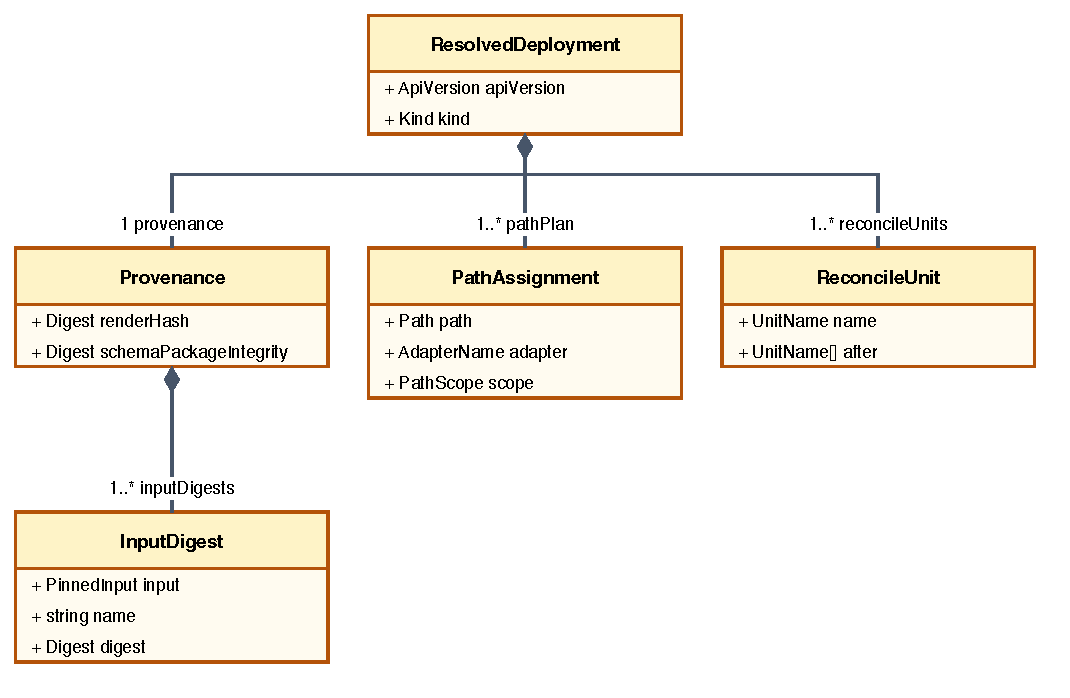
\includegraphics[width=0.92\linewidth, keepaspectratio]{Figures/t-frame}
\caption{The Estate-Wide Frame: Provenance, the Path Plan and the Units}
\label{fig:targetframe}
\end{figure}
\begin{figure}[!htbp]
\centering
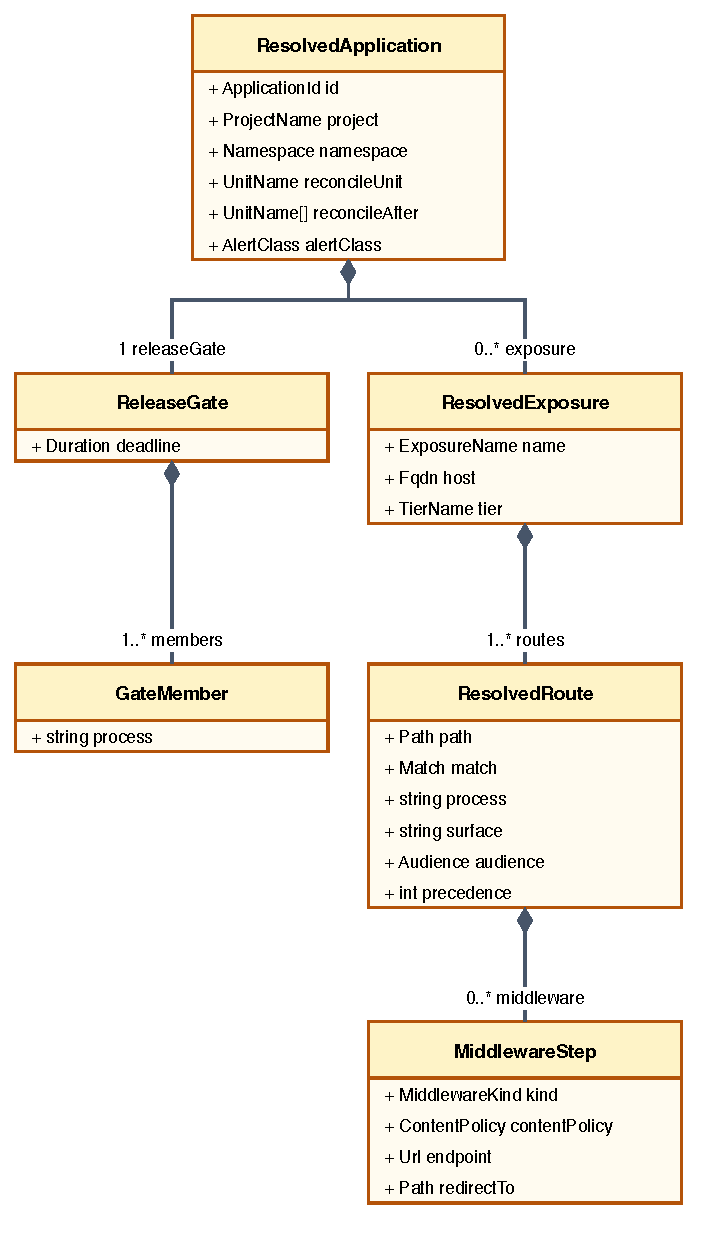
\includegraphics[width=0.92\linewidth, keepaspectratio]{Figures/t-app}
\caption{A Resolved Application: Its Release Gate, Its Migration and Its Exposure}
\label{fig:targetapp}
\end{figure}
\begin{figure}[!htbp]
\centering
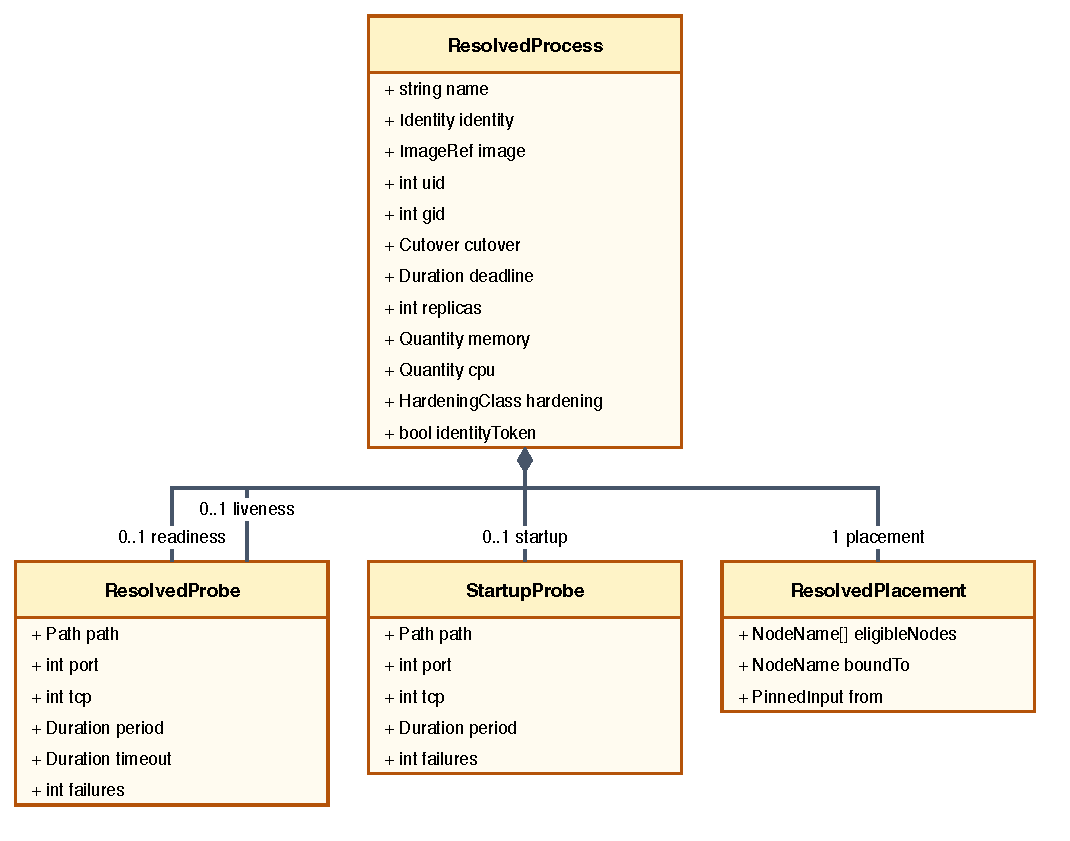
\includegraphics[width=0.92\linewidth, keepaspectratio]{Figures/t-proc-a}
\caption{A Resolved Process: Health and Placement}
\label{fig:targetprocess1}
\end{figure}
\begin{figure}[!htbp]
\centering
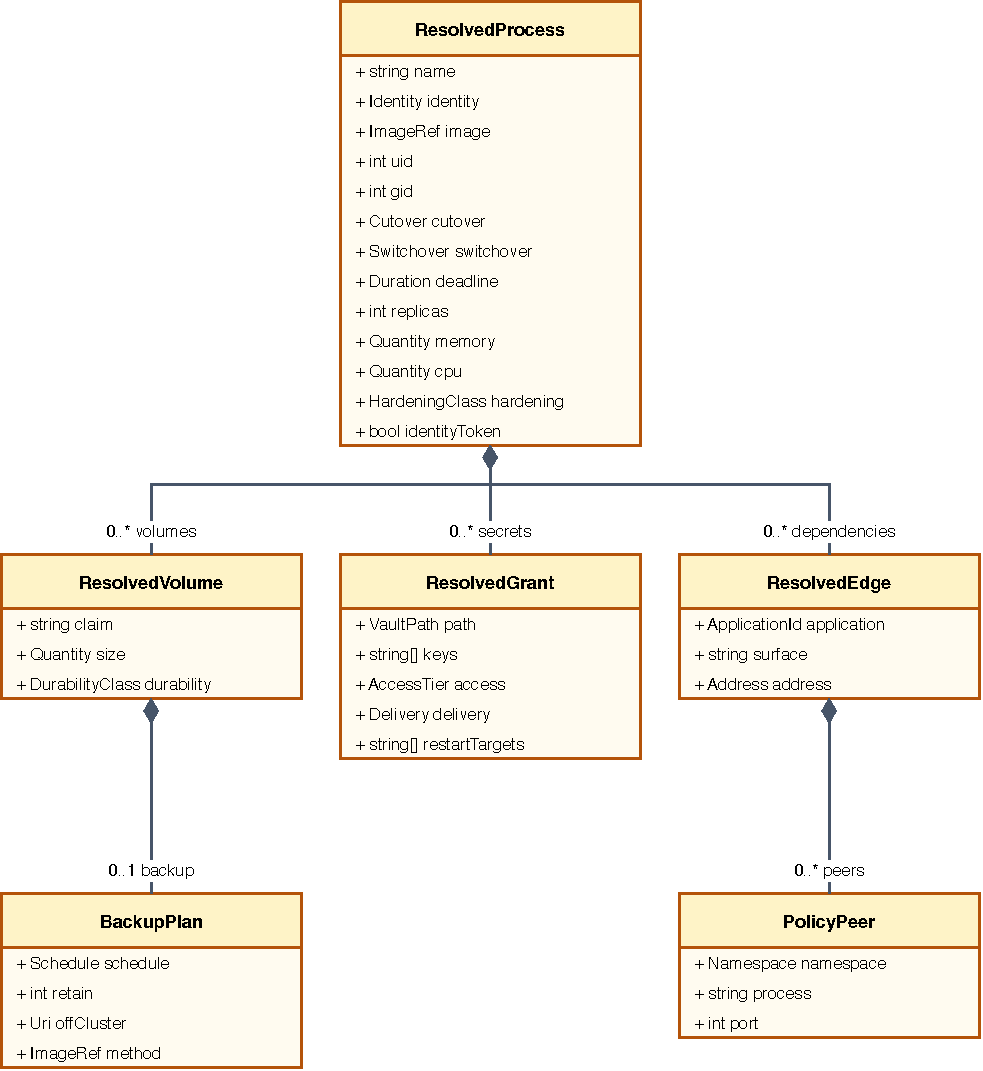
\includegraphics[width=0.92\linewidth, keepaspectratio]{Figures/t-proc-b}
\caption{A Resolved Process: Storage, Secrets and Dependencies}
\label{fig:targetprocess2}
\end{figure}
\begin{figure}[!htbp]
\centering
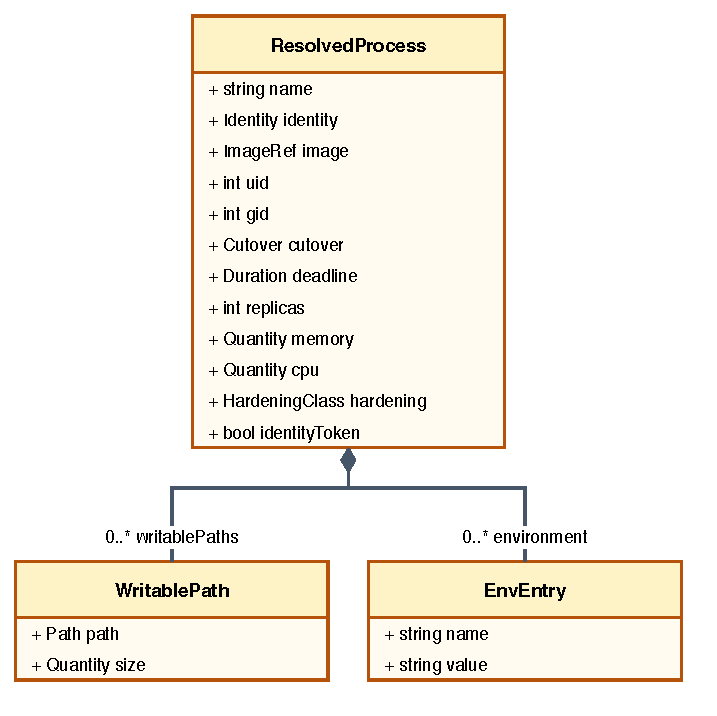
\includegraphics[width=0.92\linewidth, keepaspectratio]{Figures/t-proc-c}
\caption{A Resolved Process: Writable Paths and Configuration}
\label{fig:targetprocess3}
\end{figure}

The root is a \texttt{ResolvedDeployment} covering the whole estate, because
several of its properties are estate-wide and cannot be computed for one
application alone. It carries the provenance, the resolved applications, the
units and their ordering, and the path plan.

A \texttt{ResolvedApplication} is both the element the estate-wide model
contains and the document published back to an application's own repository. In
the second role it carries its own provenance; nested in the estate-wide model
it does not, because the enclosing document's provenance already covers it. This
is what makes the projection a filtering of the estate-wide model rather than a
second computation, so the two cannot disagree.

A \texttt{ReleaseGate} carries its \texttt{GateAnalysis} cadence and one
\texttt{GateMember} per blue/green process, and is absent wherever no process
switches blue/green: an interrupted application stops before it starts, and an
application of the delivery machinery rolls in place, so nothing waits on a
gate. A \texttt{ResolvedMigration} records only
what varies: the migration image, the revision it was tested against, and
whether the release holds a changeset that cannot run in a transaction, which no
automatic undo may touch; the identity that runs it, the owner role and the deadline are fixed functions of the
application and the platform document, so recording them would repeat a
derivation.

Below it, a \texttt{ResolvedProcess} carries the per-process decisions; its
cutover and switchover are both unset on a prepare process, which runs once and
cuts over nothing, a
\texttt{ResolvedExposure} carries the hostname with its tier, middleware chain
and ordered routes, and the volumes, grants, dependency edges and writable paths
each carry what the platform decided about them.

\subsection{The Path Plan}

Every output path is assigned here, not by the generator that writes the file.
The model carries, for each object to be generated, the generator that owns it
and the path it is written to.

The rule follows from the layer rule rather than adding to it, and two observed
cases show that the alternative does not work. An object that belongs to a group
of applications rather than to one of them is emitted once per application when
the path is computed per generator, producing several identical objects at
several paths. And an estate-wide object lands in whichever namespace the
generator that emitted it happened to key off. Assigning the paths in the model
also moves the check that two generators never claim one path to a point where
the complete set of paths is known, which is before any generator runs.

\subsection{The Generated Resources}

The generation step has a closed set of six generators, one per subsystem: the
workloads and their supporting objects, including the Canary through which a
blue/green process is switched, the network policy, the monitoring
objects, the edge routing, the secret-store policies, and the secret delivery
objects. The set being closed is the scope commitment of
Section~\ref{sec:introduction}: adding a seventh is a recorded decision, not a
new feature.

\subsection{No Target Field Names}

The constraint of Section~\ref{sec:decisions} applies most visibly here. The
resolved model records that a process switches blue/green; it does not record
a rollout strategy or a Canary: the typed resource a generator walks for it is
a \texttt{SwitchoverFile}, and only the generator spells it as a Canary. It
records the hardening posture and the
paths the process must write; it does not record a security context. It records
the middleware chain as a sequence of named steps; it does not record the target
proxy's spelling of them. Each generator is the one place its own target
vocabulary appears, and that separation is checked directly rather than left to
review.
